
%=============================================================
\subsection{A path-conservative ADER-DG scheme}\label{sec:holy-dg-scheme}
%=============================================================
The weak formulation of a first order PDE system \eqref{intro:quasi-linear} is
recast as integral equation by integrating over the control volume
$\Omega_i \times [t^n, t^{n+1}]$,
%\todo{Probably bring unter somewhere:
%This scheme is developed by the Trento group and presented in various
%papers such as \cite{Zanotti2015c,Zanotti2015c,Zanotti2015d,ADERDGVisc}
%in the context of the Euler equations of compressible
%gas dynamics, ideal MHD, special relativistic RMHD, compressible
%Navier-Stokes and viscous and resistive MHD equations.
%}%
%
\begin{equation}
 \int \limits_{t^n}^{t^{n+1}} \int\limits_{\Omega_i } \Phi_k \left[
  \partial_t \boldsymbol{Q} + \boldsymbol{A}(\boldsymbol{Q}) \cdot\nabla
  \boldsymbol{Q}
  -\boldsymbol S (\boldsymbol Q)
  \right] \,\mathrm d^d x\,\mathrm dt = 0\,, \label{eq:weakPDE}
\end{equation}
%
where $\Phi_k\in \mathcal{U}_h^N$ is a generic basis element out of the
piecewise polynomials of maximum degree $N$ which are by definition allowed
to be discontinous across the element interfaces $\partial \Omega_i$. The
resulting jump terms have to been properly taken into account.
This is done in our
numerical scheme with the aid of the path-conservative approach, first
developed by Castro and Par\'es in the finite-volume framework
\cite{Castro2006, Pares2006} and later extended also to the DG
finite-element framework in \cite{Rhebergen2008, Dumbser2009a,
	Dumbser2010}.
In this ADER-DG framework, higher order in time is
achieved with the use of an element-local space-time predictor, denoted
by $\boldsymbol{q}_h(\boldsymbol{x},t)$, which is subject to later discussion.
At this point of the deviation, the solution $Q$ will just be replaced by the
local predictor solution $\boldsymbol{q}_h=\Phi_k(\boldsymbol{x}) \boldsymbol{\hat u}^n_k$.
By integration of the first part in time, and adding a surface flux integral for
the integral over system matrix $\boldsymbol A$\footnote{
  A similar flux is not even possible for the source $\boldsymbol S$
  because it is by construction purely algebraic and must lack derivatives.
}, thus taking jumps between elements into account,
the approximation to the weak form solution \eqref{eq:weakPDE} can be written as
%
\begin{fullwidth}
\begin{align}
\label{eqn.pde.nc.gw2}
\left( \hat{\boldsymbol{u}}^{n+1}_{i,l} - \hat{\boldsymbol{u}}^{n}_{i,l} 
\right)
\int \limits_{\Omega_i}  \Phi_k \Phi_l \,\mathrm d^d x
%
+ \iint \limits_{T^n ~ \Omega_i^\circ}
 \Phi_k \left( \boldsymbol{A}(\q_h) \cdot \nabla \q_h  \right)
 \,\mathrm d^d x\,\mathrm dt
+ \iint \limits_{T^n ~ \partial \Omega_i}
 \Phi_k \mathcal{A}\left( \q_h^-, \q_h^+ \right)
 \cdot \boldsymbol{n} 
 \,\mathrm d^{d-1} x\,\mathrm dt
=
\iint \limits_{T^n ~ \Omega^\circ_i}
\Phi_k \boldsymbol{S}(\q_h)  
 \,\mathrm d^d x\,\mathrm dt
\,,
\end{align}
\end{fullwidth}
%
where the first integral is a scalar product between two basis elements
(called ``element mass matrix'', diagonal for the Legendre basis nodes), the
second integral collects the smooth part of the discrete solution in the
interiour $\Omega_i^\circ = \Omega_i \backslash \partial \Omega_i$\footnote{
  The volume integrals $\int_{\Omega^\circ}$ can be
  evaluated exactly in $N$th order with Gaussian quadrature, since all functions
  under the integral are written on the $(N+1)$th nodal basis.	
}, the third
integral collects the unsteady solution across element interfaces on the
surface $\partial\Omega$ and the fourth integral is the source term volume
integral which unterwent no special treatment thanks to the purely algebraic
nature of the source terms (lack of derivatives).

In order to distinguish the conservative and nonconservative fluxes, the
weak form \eqref{eq:weakPDE} shall be expanded again, this time by using
the PDE functions $F^i_j$ and $B^{ij}_k$ in
$\boldsymbol A = \partial \boldsymbol F / \partial \boldsymbol Q + \boldsymbol B$,
%
\begin{fullwidth}
	\begin{equation}
	\begin{aligned}
	\label{eqn.pde.nc.gw3}
	\left( \hat{\boldsymbol{u}}^{n+1}_{i,l} - \hat{\boldsymbol{u}}^{n}_{i,l} 
	\right)
	\int \limits_{\Omega_i}  \Phi_k \Phi_l \,\mathrm d^d x
	%
	&- \iint \limits_{T^n ~ \Omega_i^\circ}
	\left( \nabla \Phi_k \right) \cdot \boldsymbol F(\boldsymbol q_h)
	\,\mathrm d^d x\,\mathrm dt
	&&+ \iint \limits_{T^n ~ \partial \Omega_i}
	\Phi_k \mathcal{G}\left( \q_h^-, \q_h^+ \right)
	\cdot \boldsymbol{n} 
	\,\mathrm d^{d-1} x\,\mathrm dt
	\\
	&+ \iint \limits_{T^n ~ \Omega_i^\circ}
	\Phi_k \left( \boldsymbol{B}(\q_h) \cdot \nabla \q_h  \right)
	\,\mathrm d^d x\,\mathrm dt
	&&+ \iint \limits_{T^n ~ \partial \Omega_i}
	\Phi_k \mathcal{D}\left( \q_h^-, \q_h^+ \right)
	\cdot \boldsymbol{n} 
	\,\mathrm d^{d-1} x\,\mathrm dt
	=
	\iint \limits_{T^n ~ \Omega_i}
	\Phi_k \boldsymbol{S}(\q_h)  
	\,\mathrm d^d x\,\mathrm dt
	\,.
	\end{aligned}
	\end{equation}
\end{fullwidth}
Note that the integrals in \eqref{eqn.pde.nc.gw3} for the nonconservative matrix
$\boldsymbol B$ are the same as for the system matrix $\boldsymbol A$ in
\eqref{eqn.pde.nc.gw2}. Here, the surface integral over $\mathcal G$ was
derived rigorously by partial integration of the volume integral over
$\nabla \cdot \boldsymbol F$ and mathematically, $\mathcal G = \boldsymbol F$.
Similarly, $\mathcal D = \boldsymbol B\cdot \nabla Q$ and
$\mathcal A = \mathcal G + \mathcal D$. The curly symbols indicate approximate
Riemann solvers which depend on the boundary extrapolated states on the left
$\q_h^-$ and right $\q_h^+$ of the interface\footnote{
	Here the discontinous nature manifests, where the system state is really
	double valued (at a single coordinate).
}. In this work we mainly use the simple Rusanov flux \cite{Rusanov1961a}
%
\begin{equation}
  \mathcal{G}\left(\q_h^-, \q_h^+ \right) \cdot \boldsymbol{n} = \frac{1}{2}
  \left( \boldsymbol{F}(\q_h^+) + \boldsymbol{F}(\q_h^-) \right) \cdot \boldsymbol{n}
  - \frac{1}{2} |\Lambda_i| \left( \q_h^+ - \q_h^- \right)\,,
	\label{eq.aderdg.riemann} 
\end{equation} 
%
where $|\Lambda_i|=\max\{\max\left(\Lambda_i(\q_h^+)\right), \max\left(\Lambda_i(\q_h^-)\right) \}$ denotes the maximum wave
speed (eigenvalue) computed from both sides\footnote{Any other monotone numerical flux function could be used  equally well, see for instance \cite{toro-book} for an overview of
different Riemann solvers}. In contrast, the jump term $\mathcal D$ of the nonconservative
product follows the path-conservative approach 
\cite{Pares2006,Castro2006,Dumbser2011,DLM1995},
the jump terms are defined via a path integral (line/curve integral) in phase space
(state vector space) between the boundary extrapolated interface states
\begin{equation}
\label{eqn.aderdg.ncp}
\mathcal{D}^-\left( \q_h^-, \q_h^+ \right) \cdot \boldsymbol{n} =
\frac{1}{2} \left( \, \int \limits_{0}^1
\boldsymbol{A}(\boldsymbol{\psi}) \cdot \boldsymbol{n} \, \d s \right)
\left( \q_h^+ - \q_h^- \right) - \frac{1}{2} |\Lambda_i| \left(
\q_h^+ - \q_h^- \right),
\end{equation}
with a simple segment path $\boldsymbol{\psi} = \q_h^- + s \left( \q_h^+ - \q_h^- \right)$.
Again, the line integral can be solved on Gaussian quadrature points. Note the
similarity between the conserved \eqref{eq.aderdg.riemann} and nonconserved flux
approximation \eqref{eqn.aderdg.ncp}. It represents the extension of the Rusanov
(or local Lax-Friedrichs) flux to the nonconservative case.
Indeed, other more sophisticated schemes may be
used with the aim of reducing the numerical dissipation\footnote{see \eg the
{HLLEM}-type version of~\cite{NCP_HLLEM}, which is an extension of the
HLLEM flux of~\cite{Harten83,Einfeldt1991}, or the path-conservative Osher 
schemes
forwarded in~\cite{Dumbser2011}.}.

Several notes shall be made at this point. First, the explicit formalization of
source terms containing derivatives as ``nonconservative terms''
(Section \ref{sec:ncp}) allows to take both contributions---the algebraic and differential
sources---into account in a Riemann solver, resulting in a more exact and balanced
scheme at computationally little extra cost.
The main advantage of these path-conservative schemes is that
they allow at least in principle the construction of well-balanced
numerical schemes that are able to preserve particular steady-state
solutions of the governing partial differential equations
exactly\footnote{This is applied in Section~\vref{chapter:hydro} to the GRMHD PDE
for the first time.}. Second, it should be noted that the overall ADER-DG
scheme presented here is $(N+1)$th order accurate for smooth solutions.
Since the final algorithm is a purely {explicit} DG scheme, a
CFL-type stability condition on the time step holds in the form
\begin{equation}\label{eq.aderdg.CFL}
\Delta t_{\text{DG}} < C \frac{\Delta x }{d
  \left(2N+1\right)} \frac{1}{|\Lambda_i|} \,,
\end{equation}
with spatial patch size $\Delta x$ in $d$ spatial dimensions,
$|\Lambda_i|$ the maximal wave speed of the system, and $0<C<1$
the CFL factor, which can be chosen as large as $C=0.9$.
\footnote{For the results of a numerical 
von Neumann stability analysis of ADER-DG schemes, see \eg 
\cite{dissdumbser,QiuDumbserShu,Dumbser2008}.} 


\subsection{Local spacetime predictor} \label{sec:STDG}
%
The element-local spacetime predictor solution $\q_h(\boldsymbol x, t)$ is
computed from the known discrete solution $\u_h(\boldsymbol x, t^n)$ at
time $t^n$ using a solution of the Cauchy problem ``in the small'', \ie
within a single cell, without considering the
interaction with the neighbouring cell. For linear systems,
the Cauchy-Kovalewski procedure \cite{eno,Titarev2002,Titarev2005,Toro2006,Dumbser2007}
is suitable, it avoids a quadrature in time in favour of an iterative Taylor
series (for which the PDE system has to undergo an algebraic manipulation,
this makes its applicatioin very hard for complex systems).
For nonlinear systems, a fixed-point Picard iteration is more suitable.
\footnote{Picard's method for solving an ODE is based on
	the Picard-Lindelöf theorem, better known as Cauchy-Lipschitz theorem~\cite{AmannODE}.
	It is a simple iterative procedure which is especially suitable
	in DG due to the function base.
}
In the following, the solution is written in a spacetime basis $\q_h = \Theta_k(t,\x) \hat\u^n_k$
with $\Theta_k(t,\x)=\phi_{k_0}(\tau)\Phi(\boldmath \xi)$ the same nodal basis as before,
but including time (which is mapped to a reference time
$\tau=(t-t^n)/\Delta t \in [0,1]$). Formally the procedure of multiplying
the PDE \eqref{intro:quasi-linear} by the new test functions $\Theta_k$ and
integrating over $\Omega_i \times T^n$ yields\footnote{
	\eqref{eq:weakPDE2} is \eqref{eq:weakPDE} with $\Theta_k$ in place of 
	$\Phi_k$ and (anticipating)
	$\q_h$ in place of $\boldsymbol Q$.
}
\begin{equation}
	\iint \limits_{T^n ~ \Omega_i}
	\Theta_k(t,\x) \left[
	\partial_t \boldsymbol{q}_h + \boldsymbol{A}(\boldsymbol{q}_h) \cdot\nabla
	\boldsymbol{q}_h
	-\boldsymbol S (\boldsymbol q_h)
	\right] \,\mathrm d^d x\,\mathrm dt = 0\,, \label{eq:weakPDE2}
\end{equation}
Again, an integration by parts of the temporal derivative part is done,
but in constrast to \eqref{eqn.pde.nc.gw2} or \eqref{eqn.pde.nc.gw3},
no surface integrals are introduced since jumps are not taken into account
in this element-local prediction,
\begin{fullwidth}
\begin{multline}
\label{eqn.pde.st2}
\int \limits_{\Omega_i}   \Theta_k(\x,t^{n+1}) \q_h(\x,t^{n+1}) \d^d x -
\int \limits_{\Omega_i}   \Theta_k(\x,t^{n}) \u_h(\x,t^{n}) \d^d x
%
- \iint \limits_{T^n ~ \Omega_i}
\frac{\partial \Theta_k(\x,t)}{\partial t}  \q_h(\x,t)
\,\mathrm d^d x\,\mathrm dt
\\
=
\iint \limits_{T^n ~ \Omega_i}
\Theta_k(\x,t) \left(
\boldsymbol{S}(\q_h) - \boldsymbol{A}(\q_h) \cdot \nabla \q_h  \right)
\,\mathrm d^d x\,\mathrm dt
\,.
\end{multline}
\end{fullwidth}
\eqref{eqn.pde.st2} is now a system of $N$ indepdent element-local equation
systems (with $N$ the number of elements covering the simulation domain $\Omega$).
Each of these equations can now be solved with a (discrete) fixed-point
Picard iteration, without needing any communication with neighbour elements 
\cite{Dumbser2008,Dumbser2009a,Toro2009b,Dumbser2014}.

It should be stressed that the choice of an appropriate
initial guess $\q_h^0(\x,t)$ for $\q_h(\x,t)$ is crucial to obtain a
computationally efficient scheme.  One can either use an extrapolation
of $\q_h$ from the previous time interval $[t^{n-1},t^n]$, as suggested
in \cite{ADERPrim}, or a second-order accurate MUSCL-Hancock method, as
suggested in \cite{Hidalgo2011}. For the initial guess, one can write a
Taylor series expansion in time and then only needs to compute
approximations to the time derivatives of $\q_h$ at time $t^n$.
 A second-order accurate 
MUSCL-type initial guess for for $\q_h(\x,t)$ is given by
\footnote{Here $\partial_t u = \mathcal L(u,\partial_i u)$ is the right 
	hand side of the PDE, as in \eqref{eq:mol-ode}.}
\begin{equation} 
  \q^0_h(\x,t) = \boldsymbol{u}_h(\x,t^n) + \left(t - t^n\right)  \boldsymbol{\mathcal{L}}(\boldsymbol{u}_h(\x,t^n)), 
\end{equation} 
while a third-order accurate initial guess for $\q_h(\x,t)$ reads 
\begin{equation}
\q^0_h(\x,t) = \boldsymbol{u}_h(\x,t^n) + \left(t - t^n\right)  \boldsymbol{k}_1 + 
 \frac{1}{2} \left(t - t^n\right)^2 \frac{\left( \boldsymbol{k}_2 - \boldsymbol{k}_1 \right)}{\Delta t}, 
\end{equation} 
where $\boldsymbol{k}_1 := \boldsymbol{\mathcal{L}}\left(\boldsymbol{u}_h(\x,t^n)
\right)$ and $\boldsymbol{k}_2 :=
\boldsymbol{\mathcal{L}}\left(\boldsymbol{u}_h(\x,t^n) + \Delta t \boldsymbol{k}_1
\right)$.  For an even higher-order accurate initial guess, 
continuous extension Runge-Kutta (CERK) schemes as proposed in
\cite{OwrenZennaro} were adopted\footnote{
 For the use of CERK schemes as time integrators of
explicit discontinuous Galerkin schemes, see \cite{Gassner2011a}.}
Having an initial guess of the order $N$ chosen, it is sufficient to use
\emph{one single} Picard iteration in order to solve \eqref{eqn.pde.st2}
\footnote{
  In fact within the \code{ExaHyPE} code it was found that the $N$th order CERK 
  guess
  could dramatically improve the parallelizability of the code. This is
  because a variable-length fixed point iteration is hardly vectorizable.
}.

It should be remarked again that one-step ADER schemes, in constrast to
classical Runge-Kutta time stepping, is particular well suited for AMR
with time-accurate local-timestepping (LTS), requiring only one communication
with neighbouring cells per timestep.

\subsection{Finite-volume subcell limiter}\label{sec:limiter}

The ADER-DG scheme (\ref{eqn.pde.nc.gw3}) is formally of order $N+1$ for
smooth solutions, hence the method must be {oscillatory} for $N>0$ in the
presence of discontinuities, since the scheme is {linear} in the sense of
Godunov \cite{Godunov59}, thus inevitably generating spurious oscillations
(also known as the {``Gibbs phenomenon''}).
In order to cope with this problem, several
attempts have been made, \eg artificial viscosity
\cite{Hartman2002,Persson2006,Feistauer2013}, filtering \cite{Radice2011},
hybridisation with finite-volume/finite-difference schemes for the
selected {``troubled cells''} adopting some sort of high-order
slope-limiting procedures \cite{Cockburn1998, Qiu2004, Qiu2005, 
	Balsara2007,
	Zhu2008, Zhu2013, Luo2007, krivodonova_2007_lho}.

In this section, a finite volume subcell limiter technique shall be
prestende (first proposed in \cite{Dumbser2014}), which is based on the
multi-dimensional optimal order detection (MOOD)
\cite{Clain2011,Diot2013}. 
The main advantage of this approach is that the
high-resolution properties of unlimited DG methods are preserved thanks
to the introduction of a {subgrid level}, which is used
for integrating the partial differential equations in troubled cells by
means of a more robust high-order accurate finite-volume scheme. In the present
scheme, limiting is implemented on a \emph{per cell} basis, \ie either the
whole cell $\Omega_i$ undergoes a  treatment or no point within it. In order
to encounter this problem, adaptive mesh refinement 
(Section~\ref{sec:mesh-refinement}) is necessary to localize the limited cells
sharply around the problematic spatial region.
\footnote{
 For alternative subcell DG limiters, see also \cite{Casoni2013,
  Sonntag2014,Sonntag2017, Fechter2015, Meister2016}.
}

\subsection*{Limiting criteria}
Limiting can be applied \emph{a-priori} (before an ADER-DG time step) or 
\emph{a-poster\-iori}
(after an ADER-DG time step, as an \emph{predictor-corrector} approach). In both
cases, criteria are neccessary to decide wether limiting is neccessary. A-priori
criteria can be geometry-based
\footnote{for instance: limit in the vicinity of a spacetime singularity in a
 stationary spacetime, within the context of Einstein field equations, Section~\ref{chapter:gr}.}
or depend on the state vector.~\footnote{for instance, having reached a critical value
within an element $\Omega_i$.}

A-poste\-ri\-ori criteria test the computed \emph{candidate solution} $\u_h(t^{n+1},\x)$
on mathematical and physical admissibility criteria. Mathematical scenarios that
may violate the admissibility are the vicinity of steep-gradients or discontinuities,
under-resolved flow features or the presence of floating point errors\footnote{
	Floating point errors result in
	\emph{NaNs} (Not-a-number), a special number state within the IEE754 number
	representation which for instance occurs after dividing by zero or after
	taking the root of a negative number. Clearly, the user PDE has to be sensitive
	on such events to generate NaNs.
}. Physical admissible criteria go along with the PDE properties and can be for
instance low pressure and density conditions\footnote{
  This particular example suggests that vacuum regions in fluid dynamics should
  be limited, which is in fact not favorable at all.
}, superluminal velocities, failure
of recovering primitive variables from conserved ones (examples taken from the GRMHD,
Chapter~\ref{chapter:hydro}) or closeness to a singularity, indicated by a certain
steepness of the curvature (example from the CCZ4,
Chapter~\ref{chapter:gr}). Furthermore, the \code{ExaHyPE} code applies a
relaxed discrete maximum principle (DMP),
which checks for an unphysical steepening and reads
%
\begin{equation} 
\min \limits_{\boldsymbol{y}\in {\cal{V}}_i} (\boldsymbol{u}_h(\boldsymbol{y},t^n))-\delta \leq
\boldsymbol{u}_h(\boldsymbol{x},t^{n+1})\leq \max \limits_{\boldsymbol{y}\in
	{\cal{V}}_i}(\boldsymbol{u}_h(\boldsymbol{y},t^n))+\delta
\,, 
\label{eq:DMP}
\end{equation}
%
where ${\cal{V}}_i$ is the set containing the space-element $\Omega_i$
and its neighbours that share a common node with $\Omega_i$.
%
In \cite{Dumbser2017,Fambri2018}, we choose the parameter $\delta$ in (\ref{eq:DMP}) is as
%
\begin{equation}
\delta =\max \left( \delta_0\,, \epsilon \times \left( \max
\limits_{y\in {\cal{V}}_i}(\boldsymbol{u}_h(\boldsymbol{y},t^n))- \min
\limits_{y\in {\cal{V}}_i}(\boldsymbol{u}_h(\boldsymbol{y},t^n))\right)\,
\right)\,,
\end{equation}
with typical values $\delta_0 = 10^{-8}$ and $\epsilon = 10^{-7}$.
 
\subsection*{The coupled limiting ADER-DG scheme}
\begin{figure}[t]
	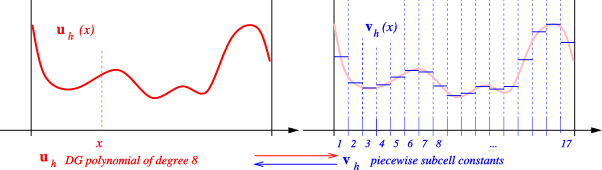
\includegraphics[width=\textwidth]{limiting-grid/limiter-P7bis-single.pdf}
	\caption[
	  Sketch of the DG-FV limiting projection/restriction,
	  \modifiedAfter{Dumbser2014,exahype-guidebook}
	]{
		A cartoon which demonstrates how a high order 
		Discontinous Galerkin solution/polynomial $u_h$ within a single patch
		(red)
		is projected onto $2N+1$ finite volume subcell averages (blue).
		The projection works in both ways, whereas the one from the higher
		amount of degrees of freedom (FV limiter) is called \emph{restriction}.
		Figure modified from
		\cite{Dumbser2014,exahype-guidebook}.
	}\label{fig:aderdg-limiter-2np1}
	% Is the citation correct? It was Dumbser2014b before.
\end{figure}
	
 In practice, each
 computational cell $\Omega_i$ that has been marked for limiting is split
 into $(2N+1)^3$ finite-volume subcells, which are denoted by
 $\Omega_{i,s}$ and that satisfy $\Omega_i = \bigcup_s \Omega_{i,s}$ (see
 Fig. \ref{fig:aderdg-limiter-2np1}). Note that this very fine division of a DG
 element into finite-volume subcells does \textit{not} reduce the timestep
 of the overall ADER-DG scheme, since the Courant-Friedrichs-Lewy (CFL)
 coefficient of explicit DG schemes scales with $1/(2N+1)$, while the CFL
 of finite-volume schemes (used on the subgrid) is of the order of
 unity \cite{Dumbser2014,Zanotti2015c,Zanotti2015c,Zanotti2015d,ADERDGVisc}.
 The discrete solution in the subcells $\Omega_{i,s}$ is
 represented at time $t^n$ in terms of \textit{piecewise constant} subcell
 averages $\bar{\u}^n_{i,s}$, \ie \footnote{as in Godunov's scheme,
 	eq. \eqref{eqn.subcellaverage} }
 %
 \begin{equation}
 \bar{\u}^n_{i,s} := \frac{1}{|\Omega_{i,s}|} \int \limits_{\Omega_{i,s}}
 \Q(\x,t^n) d \x\,.
 \end{equation}
 %
 These subcell averages are evolved in time with any {suitable}
 finite-volume scheme. \footnote{See Section~\ref{sec:fv} for a presentation of
   finite volume schemes. The \code{ExaHyPE} paradigm to decide
   \emph{suitability} is to assume that robust finite volume methods for
   a given problem are understood and can be used as a safe \emph{fallback}
   in case of problematic DG solutions which require limiting.
 } 
 
 In fact, the limiting ADER-DG (or: hybrid) scheme can be understood as
 a DG solver  coupled to a FV solver, acting on the same grid. To do so,
 on a limited patch, the ``embedded'' DG quadrature points are replaced by
 an equally embedded finite volume grid. The resulting limited 
 finite volume patch has a block-regular structure of $(2N+1)$
 cells (see Section~\ref{sec:block-regular-grids} about block regular grids). 
 
 From the finite volume scheme, a new piecewise constant solution $\boldsymbol{v}_h(\x,
 t^{n+1})$ given by the cell averages $\bar{\boldsymbol{v}}_{i,s}^{n+1}$
 is obtained, from which the final, {limited} DG
 polynomial as $\boldsymbol{u}_h(\x,t^{n+1}) = \mathcal{R}\left( \boldsymbol{v}_h(\x,t^n) \right)
 $ is reconstructed, where $\mathcal{R}$ is the reconstruction operator associated with the
 projector $\mathcal{P}$, so that $\mathcal{R} \circ \mathcal{P} =
 \mathcal{I}$, with $\mathcal{I}$ the identity operator \cite{Dumbser2014}.
 %
 For the subcell finite-volume scheme a different CFL stability condition
 applies and takes the form
 \begin{align}
 \Delta t_{\text{FV}} < \text{CFL}\frac{h_{\text{min}}}{d \, N_s}
 \frac{1}{|\lambda_{\text{max}}|}, \label{eq:CFLweno}
 \end{align}
 with $h_{\min}$ the minimum cell size referred to the DG control volumes
 $\Omega_i$ and $\lambda_\text{max}=|\Lambda_i|$ the maximal wave speed of the
 system. Choosing $N_s \geq N+1$ is a natural requirement that allows
 to reconstruct the of degrees of freedom of $\boldsymbol{u}_h$ from the piecewise
 constant solution $\boldsymbol{v}_h$ via $\mathcal{R}$. Following \cite{Dumbser2014}
 we choose $N_s = 2N + 1$ so that $\Delta t_{\text{FV}} = \Delta
 t_{\text{DG}}$. This choice allows us to maximise the resolution
 properties of the chosen subcell finite-volume scheme and to run it at
 its maximum possible CFL number. 


When considering time integration, in ADER schemes for nonlinear hyperbolic PDE,
limiters need to be applied only once per time step, while in Runge-Kutta based 
MoL schemes, the limiter needs to be applied in each Runge-Kutta 
stage again \footnote{
    For a detailed comparison of Runge-Kutta and ADER
	finite-volume schemes, see \cite{dumbser_diffapprox} and
	\cite{Balsara2013}, while Runge-Kutta DG and Lax-Wendroff DG schemes
	(the latter are very similar to ADER-DG schemes) have been compared in
	\cite{QiuDumbserShu}, also concerning computational performance. Detailed
	computational performance comparison between ADER-DG schemes and RKDG
	schemes are also given in Appendix~\vref{sec:rkdg-performance}.}.

%=============================================================
%\newpage % for simplicty with the figures here
\section{Grid meshing}\label{sec:grid-meshing}
The issue of storing the data necessary for the presented numerical schemes is
tightly coupled to the representation of the numerical grid on the computer. This is
a technical challenge continously addressed by computer scientists, since computer
architectures are evolving in time and different aspects get important.

In this section, a couple of aspects are presented in a generic fashion, \ie there
is no particular focus on FD, FV or DG methods and it is left open what the grid
actually holds (point/vertex data, cell averages or cells with a subcell structure).

\subsection{Block regular grids}\label{sec:block-regular-grids}
\begin{marginfigure}
	\includegraphics[width=\linewidth]{numerics-grids/cactus-components.png}
	\caption[
	  Sketch of Carpet grid covering, \modifiedAfter{carpet_web}]%
	{A height-elevated plot of a scalar field on a two-dimensional domain. The displayed
	 grid structure reveals a unigrid layout. Multiple patches are shown which cover the
	 physical domain, each having the same resolution $\Delta \vec x$. Color is used
	 to distinguish the patches. Furthermore, the overlapping ghost zones are displayed
	 in a different colour. Figure modified from~\cite{carpet_web}.}%
	\label{fig:numerics-cactus-components}
\end{marginfigure}
%
The simplest grids are \emph{regular} (or \emph{uniform}, also refered to as \emph{unigrid}),
that means each grid coordinate
\begin{equation}
\vec x = \sum_{i=0}^d x_i \Delta x^i
\end{equation}
can be described by the constant vector of grid spacings $\Delta \vec x \in \mathbb{R}^d$ and
integer position indices $\vec x \in \mathbb{N}^d$. Therefore, a finite domain grid is fully
characterized
by the grid spacings $\Delta \vec x$ and a description of the domain, for instance
$\vec x = \vec x_0 + x_i \Delta x^i$ with offset $x_0$ and $x_i \in [0,N]^d$ with $N$
being the number of points.

Uniform grids can be Cartesian (unit squares, $\Delta x^i=\Delta x~\forall i\in[1,d]$)
or rectilinear (all $\Delta x^i$ may be different from each other). They also may be
curvilinear, for instance in a cylindrical or spherical coordinates mapping.
In contrast, irregular grids are called \emph{unstructured} and a priori a list of all
grid points must be stored.

Figure \ref{fig:numerics-cactus-components} shows the grid structure in an exemplaric setup
how it is used by the \code{Carpet} code, which is part of the \code{EinsteinToolkit}
\footnote{See appendix \vref{apx.codes} for details about the codes referenced in the main text.}.
Carpet implements block regular grids, \ie each of the displayed three blocks is a regular grid.
In practice, different blocks are evolved in time by different processors/computers.
For the implementation of the particular FD/FV scheme, exchange of information at the boundaries
of each block is neccessary, which is faciliated by a small overlap of the patches. Cells within
the overlapping region are called \emph{ghost cells}. Figure \ref{fig:numerics-cactus-components}
shows one layer of ghost cells around each block.

%Implementing block regular grids is an old technique and was already done 50 
%years ago.

\subsection{Mesh refinement}\label{sec:mesh-refinement}
\begin{marginfigure}
	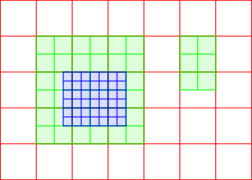
\includegraphics[width=\linewidth]{numerics-grids/Carpet-FMR.pdf}
	\caption[Carpet FMR region sketch, \colorizedAfter{Schnetter-etal-03b}]%
	{Multiple Fixed Mesh Refinement layers (FMR) in Carpet, from \cite{Schnetter-etal-03b}}%
	\label{fig:numerics-cactus-fmr}
\end{marginfigure}
%
\begin{marginfigure}
	\includegraphics[width=\textwidth]{numerics-grids/quadtree.png}
	\caption[
	AMR vs unigrid in 2D, cartoon, \modifiedAfter{Sortino2009quadtree}]%
	{   Resolving a curve in a unigrid ($16\cdot 24=384$ elements) vs.
		a local mesh refinement (quadtree, $6+12+48+96=166$ elements)
		with the same resolution, but only 43\% storage.
		Adopted from \cite{Sortino2009quadtree}.}\label{fig:amr-motivation}
\end{marginfigure}
%
Grid codes implement mesh refinement in order to resolve local features while being able to
evolve a large spatial domain. As refinement layers are supposed to have smaller cells, they also
have smaller maximum timestep sizes (due to the CFL condition). A code with \emph{global time
stepping} evolves all refinement levels with the maximum timestep size of the finest layer,
this typically leads to numerical dissipation in the coarser layers and is very slow, as
the coarser layers allow bigger timesteps. Therefore, a proper refinement code implements
\emph{local time stepping} where each refinement level is evolved with the maximum time step
possible locally. Depending on the scheme and implementation, this requires prolongation 
(projection of field values from the finer to the coarser levels) and restriction
(projection of field values from the coarser to the finer levels)
in order to make use of the finer resolved data at the different time levels.

The \code{Carpet} code implements \emph{Fixed} Mesh Refinement (FMR),
also refered to as \emph{moving boxes} or \emph{boxes in boxes}. The concept is visualized
in Figure \ref{fig:numerics-cactus-fmr} where three refinement levels are displayed (here
without ghost zones). Refinement layers can be ordered by their resolution, this motivates
to collect them in tree-structures \cite{Khokhlov98}.
Typically, codes restrict to a single refinement factor $k$.
Given a numerical scheme with convergence order $\alpha$, the convergence (refinement)
factor of the overall code will be $k\alpha$.

The dynamical version of FMR is Adaptive Mesh Refinement (AMR), where the refined areas are
created, moved and destroyed by a criterion such as a treshold on a degree of freedom
(Figure~\ref{fig:amr-motivation}).

Dynamical load-balancing (of a dynamical AMR grid) is an open research problem in
computer science. A difficulty is to detect load inequalities, moving load between nodes
and assessing the effectiveness of such an expensive operation. A code with \emph{static}
load balancing (of a static AMR problem) can circumvent this in advance by hand-crafted
distribution of work.

\begin{marginfigure}
	\includegraphics[width=\textwidth]{grmhd-paper-official/AMR_levels.pdf}
	\caption[Space-Tree illustration, TikZ figure \by{Fambri},
	  \publishedIn{Fambri2017}]{The
		\emph{space-tree} structure of the refinement levels for a single
		element at the coarsest level $\ell_0$ is shown, corresponding to the
		choice $\mathcal{R}=3$. Figure published in \cite{Fambri2017}. }
	\label{fig:numerics-AMR-single-cell}
\end{marginfigure}
%
Further aspects of mesh refinement are the starting paradigm: For instance,
being a sane Octree code, the \code{ExaHyPE} code refines from a \emph{single cell},
that is, it is an AMR code by heart (Figure \ref{fig:numerics-AMR-single-cell}).
In contrast, the \code{ExaHyPE} prototype codes as well as \code{Cactus} start with 
an already refined unigrid. At startup,
this allows for Cartesian slicing which minimizes the surface of the
blocks right at the beginning but postpones the load balancing problem to later
refinement steps.

\subsection{Parallelization}
\begin{marginfigure}
	\includegraphics[width=\linewidth]{peano-task-graphs/tasks.pdf}
	\caption[
	  Idealized ExaHyPE/Peano task graph. Modiefied from \cite{exahype-review}.
	]{
		Idealized parallel task graph in \code{ExaHyPE}.
		Modified from \cite{exahype-review}.
	}\label{fig:exahype-task-graph}
\end{marginfigure}
Hyperbolic laws with finite wave speeds invite to parallelize on the spatial
domain. Modern codes need to exploit parallelism on several hierarchies. On the
programming level, the HPC landscape is dominated by shared and distributed memory
parallelization (MIMD, multiple instruction, multiple data) as well as vectorization
(SIMD, single instruction, multiple data).
%The approach taken here distinguishes all codes mentioned so far from each other most.

The \code{Cactus} framework manages the distributed memory parallelization internally by
splitting up the simulation domain. The split follows a traditional Cartesian
domain composition. In \code{Cactus}, program modules (\emph{thorns}) 
allow for random read
and write access to the grid, have to describe the numerical schemes and the physics
(PDEs). They need to implement shared memory parallelization as well as
vectorization.
In contrast, the \code{ExaHyPE} framework manages both distributed and shared memory
parallelization, so that users are only confronted with providing their PDE in a
vectorizable way \footnote{
 Section \ref{sec:fo-ccz4-implementations} provides a discussion of
 vectorized implementations of the CCZ4 formulation of Einsteins Equations.}.
Being an active research code for AMR, \code{ExaHyPE} implements a number
of state-of-the-art domain
decomposition paradigms, for instance it dimensionally reduces the computational domain
by \emph{domain filling curves}, thus mapping physical locality to memory locality.
This is useful for hyperbolic conservation laws where causality implies that significantly
seperated spatial regions do not influence each other.
The mesh code in \code{ExaHyPE} is called \code{Peano} (like the spacefilling curve)
and uses two coupled state machines (finite automata) 
to couple a numerical scheme to the grid traversal
(Figure \ref{fig:peano-finite-automata}). This formalization
allows to optimize the code in numberous ways (such as doing research on task
based graphs, Figure \ref{fig:exahype-task-graph})
but locks down the
scheme to the predefined actions, prehibiting random access and
attemps done in classical codes \cite{Weinzierl2015}. This paradigm is called
``principle of loosing control'' (or ``Hollywood principle'', ``inversion of
control'') and is typical for application frameworks.

\begin{marginfigure}[-2cm]
\makebox[\linewidth][c]{% centering figure
	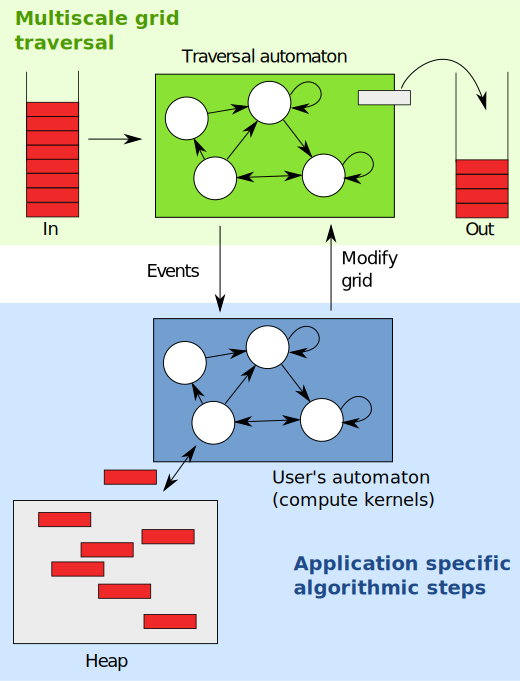
\includegraphics[width=1.05\linewidth]{peano/automata-less-width.pdf}
}% end makebox
	\caption[
  	  Finite state machines of Peano, \modifiedAfter{Weinzierl2015} 
  	%arXiV:1506.04496
	]{Cartoon of the \code{Peano}/\code{ExaHyPE} architecture.
	  Figure modified from~\cite{Weinzierl2015}.}
	\label{fig:peano-finite-automata}
\end{marginfigure}

\subsection[ADER-DG $hp$-refinement]{$hp$-refinement with ADER-DG and subcell 
limiter}
The ADER-DG algorithms with subcell finite-volume limiter described above
has been here implemented on spacetime adaptive Cartesian meshes. Details
on the used AMR algorithm are described in
\cite{AMR3DCL,Zanotti2015c,Zanotti2015c,Zanotti2015d,ADERDGVisc}.
The AMR strategy adopted is named
\emph{cell-by-cell} refinement and consists in providing a space-tree data
structure \cite{Khokhlov98, Peano1, Peano2, AMR3DCL},
whose \emph{leaves} correspond to the spatial elements $\Omega_i$ used by
the numerical scheme described before. The main alternative to a
space-tree data structure is the use of  \emph{patches},
\cite{Berger-Oliger1984, berger85, Berger-Colella1989}, where a
set of independent overlaying Cartesian sub-grid domains (or patches)
is introduced and activated when necessary. In the AMR approach used in
\code{ExaHyPE}, the numerical solution is checked independently along every single
space-element for an eventual recursive refining or recoarsening
process.
%
In practice, starting from an initial Cartesian grid of refinement level
$\ell=\ell_0=0$, which is the basic mesh without refinement, the
tree-type infrastructure of finer {refinement levels} is made
accessible. The refinement levels $\ell>0$ are built according to the so
called {refinement factor} $\mathcal{R}$, which is the number of smaller
space-elements per space-direction in which a coarser element is broken
in a refinement process, or which are merged in a recoarsening
stage. Note that choosing a refinement factor $\mathcal{R}=2$ would
generate the well known \emph{quadtrees} in two-dimensional (2D) meshes and
\emph{octree} in 3D meshes. For an arbitrary refinement factor
$\mathcal{R}$, general space-trees are obtained \cite{Peano1,Peano2}.

\begin{marginfigure}
  \includegraphics[width=\textwidth]{grmhd-paper-official/AMR_DGSubcell.pdf}
  \caption[
     AMR and DG cartoon, drawn \by{Fambri}, \publishedIn{Fambri2017}
    ]{An example of combination of AMR and DG subcell
    reconstruction is shown. The limited cells ($\beta=1$)
    $\mathcal{C}_n$ and $\mathcal{C}_m$ are highlighted in red. The
    simplest way for the polynomial reconstruction between
    $\mathcal{C}_n$ and $\mathcal{C}_m$ elements is: (i) project the
    piecewise constant solution from $\mathcal{C}_n$ to the virtual
    child-element $\mathcal{C}_v$ (see Fig.~\protect\ref{fig:AMRmaps}); (ii) do
    polynomial reconstruction along the same refinement level, between
    $\mathcal{C}_v$ and $\mathcal{C}_m$.
    Figure published in \cite{Fambri2017}.
    }
  \label{fig:AMR}
\end{marginfigure}

For practical purposes, a finite number of refinement levels is provided,
\ie from the coarser $\ell = \ell_0$ to a finest possible refinement
level $\ell = \ell_{\text{max}}\in{\rm I\!N}^+_0$. The
refinement/recoarsening process is driven by the standard \emph{Loehner scheme}
\cite{Loehner1987}, \ie a prescribed {re\-fine\-ment-estimator function}
\begin{equation}
\chi(\varphi) =
\sqrt{	\frac{
		\sum_{k,l} \left( \partial_l \partial_k \varphi \right)^2
		}{
		\sum_{k,l} 
		  \left(
          \frac{
			\left| \partial_k \varphi \right|_{i+1} + \left| \partial_k \varphi \right|_i
		  }{\Delta x_i}
		  + \epsilon
		  \left| \partial_k \partial_l \left| \varphi \right| \right|
		  \right)^2
		}
}
\end{equation}
which is a function of discrete gradients and second derivatives of a scalar
\emph{indicator function}
${\varphi}= \varphi\left(\boldsymbol{u}_h(\x,t^n)\right)$
and by two thresholds $\chi^+$ and $\chi^-$
\cite{Loehner1987,Zanotti2015d,ADERDGVisc}. Elements are
marked for refinement whenever $\chi > \chi^+$ and for recoarsening
whenever $\chi < \chi^-$. Examples for the indicator function $\varphi$
in hydrodynamics are the rest mass density ($\varphi=\rho$), production
of entropy \cite{PS:entropy, SCR:CWENOquadtree, CS:epsweno}, the Lorentz
factor, as well as geometric criteria ($\varphi=\varphi(\vec x)$).

To simplify the AMR algorithm, two neighbour elements are allowed to
belong either to the same level $\ell$ or to an adjacent refinement level
$\ell \pm 1$. To each element in the tree we assign a basic {element
  status} which is
%
\begin{align}
\sigma_i &= \left\{\begin{array}{rcl} 
-1\,, & & \text{for the  \emph{parent cells}} \\
\phantom{-}0\,, & & \text{for \emph{active elements}} \\
+1\,, & & \text{for the  \emph{virtual children}}
\end{array}\right. \nonumber \\
 i&=1,\ldots, N_{\text{tot}},
\end{align}
%
where $N_{\text{tot}}$ is the total number of space-elements present in
the tree. Note that $N_{\text{tot}}$ should be distinguished from the
total number of {active} elements $N_E$, which are the leaves of the tree
that define the $\Omega_i$ used in the numerical scheme, and for which
$N_{\text{tot}}>N_E$ holds in general. The  {parent cells}
($\sigma_i=-1$) are those tree elements which contain active elements on
a higher level and finally a {virtual child cell} ($\sigma_i=+1$) is a
tree element which is {contained} within an active cell that belongs to a
{lower} and {adjacent} refinement level $\ell-1$.

\begin{figure}[t]
\includegraphics[width=\textwidth]{grmhd-paper-tikz/standalone-AMR_maps.pdf}
\caption[
   Restriction and projection with AMR, drawin \by{Fambri},
   \publishedIn{Fambri2017}
 ]{Mapping of the numerical solution between the piecewise
  polynomials $\boldsymbol{u}_h$ of the DG scheme and the piecewise constant data
  $\boldsymbol{v}_h$ of the finite-volume scheme as well as between two different
  AMR-levels $\ell$ and $\ell+1$. Figure published in \cite{Fambri2017}.}
\label{fig:AMRmaps}
\end{figure}

Apart from the storage of flux contributions from neighbour cells within
our high-order time-accurate local time stepping (LTS) algorithm
\cite{AMR3DCL}, virtual cells are also needed for high-order
finite-volume schemes to provide the necessary data for polynomial
reconstructions (TVD, WENO) on a given refinement level if two adjacent
active cells belong to {different} refinement levels; this is illustrated
schematically in Fig. \ref{fig:AMR}. This strategy produces a locally
uniform grid around each cell and greatly simplifies reconstruction. Our
strategy of generating a locally uniform grid around each cell is very
different from the approach based on genuinely multidimensional CWENO
reconstructions proposed by \cite{SCR:CWENOquadtree}.

The dynamics of the numerical solution on virtual elements is given by
standard $L_2$ projection (for virtual children) or averaging (for parent
cells), as depicted in Fig. \ref{fig:AMRmaps}, where the mapping between
the chosen solution spaces, piecewise polynomial (unlimited) or
piecewise constant (limited), and between two adjacent refinement levels
$\ell$ and $\ell+1$ is depicted.

Due to the possibility of handling a large range of spatial
scales within the same domain, corresponding to very different CFL time
restrictions, a time-accurate and fully conservative {local time
  stepping} (LTS) has been implemented in order to use the smallest
admitted timestep only where necessary, and a large timestep where it is
allowed \cite{AMR3DCL}.

Within the \code{ExaHyPE} code, the adaptive mesh refinement can further
be triggered by the finite volume subcell limiter, which is always applied
at the finest AMR level of the simulation. In such a case, a padding is
applied around the limited regions
\cite{exahype-review,exahype-guidebook}.

%
